\documentclass[10pt,twocolumn,letterpaper]{article}

% My own stuff
\usepackage{booktabs}
% \usepackage{caption}
% \captionsetup[table]{skip=8pt}   % Only affects tables
\usepackage{stfloats}  % Add this to the preamble
\usepackage{float}
\usepackage{xeCJK}  % Supports Simplified & Traditional Chinese

\usepackage{cvpr}
\usepackage{times}
\usepackage{epsfig}
\usepackage{graphicx}
\usepackage{amsmath}
\usepackage{amssymb}

% Include other packages here, before hyperref.

% If you comment hyperref and then uncomment it, you should delete
% egpaper.aux before re-running latex.  (Or just hit 'q' on the first latex
% run, let it finish, and you should be clear).
\usepackage[breaklinks=true,bookmarks=false]{hyperref}

\cvprfinalcopy % *** Uncomment this line for the final submission

\def\cvprPaperID{****} % *** Enter the CVPR Paper ID here
\def\httilde{\mbox{\tt\raisebox{-.5ex}{\symbol{126}}}}

% Pages are numbered in submission mode, and unnumbered in camera-ready
%\ifcvprfinal\pagestyle{empty}\fi
\setcounter{page}{1}
\begin{document}

%%%%%%%%% TITLE
\title{ECDO 数据驱动入门 第一部分:当前对放热的地幔-地核解耦詹尼别科夫振荡(ECDO)“地球翻转”理论的理解}

\author{Junho\\
网站:\href{https://sovrynn.github.io}{sovrynn.github.io}\\
ECDO 研究资料库:\href{https://github.com/sovrynn/ecdo}{github.com/sovrynn/ecdo}\\
{\tt\small firstauthor@i1.org}
}

\maketitle
%\thispagestyle{empty}

%%%%%%%%% ABSTRACT
\begin{abstract}
在 2024 年 5 月,一位化名为 “The Ethical Skeptic” \cite{0} 的在线作者分享了一项突破性的理论,称为放热的地幔-地核解耦詹尼别科夫振荡(ECDO)\cite{1}。这个理论提出,地球曾经经历过突然的灾难性旋转轴移动,触发了由于旋转惯性导致的巨大的全球洪水。此外,它还提出了一种解释性地球物理过程和数据,指出可能会有另一场类似的翻转即将发生。虽然此类灾难性洪水和末日预测并不新鲜,但 ECDO 理论因其以科学、现代、多学科和数据为基础的方法而独具吸引力。

本文是为期六个月对 ECDO 理论独立研究的两部分总结的第一部分\cite{2,20},重点强调了三个关键点:

\begin{flushleft}
\begin{enumerate}
    \item 类似 ECDO 的“地球翻转”在人类近期历史上已经发生过多次,有洪水神话和广泛大陆洪水的地质迹象为证。
    \item 可以确定过去地球翻转的大致方向和幅度。
    \item 最近的地磁和地球物理数据表明另一场地球翻转可能即将发生,并且气候变化可能是由地球深处的变化而非人为活动引起。
\end{enumerate}
\end{flushleft}

此外,我还会介绍 ECDO 理论提出的“地球翻转”的原因物理学。

在本文中,我通过专注于硬数据来保持客观性,避免对理论中引人注目但具有推测性的部分进行详述,并强调这是一个人类迫切需要进一步研究的话题。
\end{abstract}

%%%%%%%%% BODY TEXT
\section{介绍}

大洪水的故事不是新鲜事——事实上,世界各地的每个主要文化中都存在这样的故事,涵盖了所有文明的摇篮。绘制(图\ref{fig:1})汇编的 267 个洪水故事 \cite{3} 显示,几乎所有有人居住的地球区域都有洪水的故事。

\begin{figure}[h]
\begin{center}
   \includegraphics[width=1\linewidth]{b.png}
\end{center}
   \caption{世界各地洪水故事的位置 \cite{3}。}
\label{fig:1}
\label{fig:onecol}
\end{figure}

仔细观察这些洪水故事,我们可以发现这些并不是普通的洪水,而是伴随着洪水的破坏性灾难,彻底清除大陆。

\subsection{美洲原住民的灾难故事}

美洲原住民的故事中包含了一些关于地球重大灾难的生动描述。居住在亚利桑那州东北部的霍皮族,一个美洲原住民部落,他们说,\textit{"…Sótuknang召唤蚁人打开他们的地下世界给被选中的人。当他们安全地在地下时,Sótuknang命令双胞胎Pöqánghoya和Palöngawhoya离开他们在世界轴心的南北两端的岗位,他们被安置在那里以确保地球正常旋转。 \textbf{双胞胎刚刚离开他们的岗位,世界失去控制,失去平衡地疯狂旋转,然后翻滚了两次。}山脉以巨大的飞溅沉入海中,海洋和湖泊漫过陆地;而当世界旋转过冷而无生气的空间时,冻结成固体冰"} \cite{4}。

这些故事中许多精确描述了洪水的巨大规模,叙述了海洋如何上升至淹没除最高山峰以外的一切。生活在华盛顿州的Skokomish印第安人讲述,\textit{"大灵对人和动物的邪恶感到愤怒,决定除去除好动物,一个好人及其家人以外的所有生命。在大灵的指示下,这位男子向云射出了一支箭,然后在那支箭上又射出了另一支箭,如此这般,从云到地面形成了一条箭的绳子。好动物和人们爬上去。坏动物和蛇开始往上爬,但那人折断了绳子。 \textbf{然后大灵造成了多日的降雨,水淹到了Takhoma(雷尼尔山)的雪线。}所有坏人坏动物都被淹死后,大灵停止了降雨,水位慢慢下降,好人和好动物爬下来了"} \cite{3}。需要参考的是,雷尼尔山是华盛顿的一座活火山,海拔高达4392.5米。

来自华盛顿州玛卡印第安人的洪水故事特别提到了一个 "非常温暖" 的多阶段洪水,这表明这不是一场普通的洪水:\textit{"海洋上升到足以切断海角。然后退去,四天后达到最低点,使Neah湾高而干燥。然后它再次上升,覆盖了除山顶以外的所有地方。 \textbf{上升的水非常温暖。} 划着独木舟的人们装上他们的物品,被送到了很远的北方。许多人在他们的独木舟被树木困住时死去。四天后,海洋恢复正常,人们发现自己远在北方,那里他们的后代仍然生活着"} \cite{3}。

\subsection{中国的灾难故事}

在太平洋的另一边,现代的中国文明据说始于一场大洪水。约公元前2000年的夏朝,由治愈了鲧禹大洪水的大禹建立 \cite{6}。在他的时代,\textit{"...据说出现了这样的奇迹:太阳在十天内没有落下,森林被点燃,众多可憎的害虫被滋生...... 一波"到达天际"的巨大波浪落在中国的土地上。\textbf{"水涨到了高山之上,连山脚都根本看不见了"}... "洪水的泛滥是毁灭性的,"皇帝说。 "它们的广泛程度覆盖了小丘,淹没了巨大的高地,用洪水威胁着天空。" 皇帝下令竭尽全力打开被困在山间峡谷中的水的出口。多年来,人民努力工作,通过挖掘渠道和排水田地来试图清除平原和山谷的洪水。许多年所有的努力都是徒劳的。负责这项迫切而巨大的工作的部长鲧,因为失败被判处死刑......只有他的儿子禹成功地排干了土地。这一成就被高度评价,在舜继任之后,禹成为中国的皇帝"} \cite{5}。

似乎不仅中国被洪水淹没了,而且需要重新测量主要方向以及太阳和月亮的运动,这暗示地球在洪水期间可能发生了旋转变动:\textit{\textbf{"这位帝王派遣学者前往中国各地,甚至到印度支那,通过观测太阳的升起和落下方向以及恒星的运动来确定北、西、东、南的位置。} 他还令他的天文学家发现季节的持续时间,并编制新的历法... "于是尧[Yaou]命令河和霍,恭敬地根据浩渺的天计算并描绘太阳、月亮、星星和黄道空间的运动和外观;并向人民恭敬地传达季节""} \cite{5}。

中国历史上关于灾变的记录实际上远早于夏朝,早到三皇五帝时期 \cite{7}。女娲,作为三皇之一也是中国历史上一位重要的创造人物,在一个地球转动改变的灾难中阻止了洪水:\textit{"两个更为强大的神之间发生了争执,他们决定通过战斗来解决。当水神共工看到自己要输时,便以头撞向不周山,这是一根支撑天空的柱子。\textbf{柱子倒塌导致天空向西北倾斜,而地面则向东南移动。} 这引发了巨大的灾难,如无尽的火灾、巨大的洪水和凶猛的食人野兽的出现。女娲砍下巨龟的腿,用来替代倒下的柱子,缓解了局势,并用七种颜色的石头封住破裂的天空,但她无法完全纠正倾斜的天空"} \cite{8}。

\subsection{欧洲、玛雅、中东及东南亚洪水传说}

由于本文中灾变故事过多,难以详细描述,我将简要提及一些其他有此类故事的著名文化。希腊文学包含三个洪水故事,即丢卡利翁、奥吉吉斯和达达努斯\cite{9,10}。在前者中,\textit{“在九天的洪水之后,世界被摧毁,方舟停在帕尔那索斯山顶”},其峰顶海拔为2,457米\cite{11}。玛雅文学认为在当前太阳之前有四个不同的太阳,第四个太阳Calchiuhtlicue的时代于公元前3100年左右以一场毁灭世界的洪水结束,并出现了当前的第五个太阳 \cite{12}。在中东,《圣经》记载了著名的诺亚洪水,《吉尔伽美什史诗》则是巴比伦叙述了类似的故事\cite{13}。东南亚文化也充满了洪水故事—例如,印度尼西亚的奥特达努姆人说,\textit{“一次大洪水曾淹没许多人。少数人通过乘船逃到唯一高出水面的山峰上而幸存。他们在那儿住了三个月,直到洪水消退”}\cite{3}。他们居住的婆罗洲岛,其最高峰海拔为4,095米。

\begin{figure*}[t]
\begin{center}
% \fbox{\rule{0pt}{2in} \rule{.9\linewidth}{0pt}}
\includegraphics[width=1\textwidth]{marine.jpg}
\end{center}
   \caption{全球海洋化石、咸水和盐滩/矿井分布图\cite{15,16,86,87}。}
   \label{fig:2}
\end{figure*}

\subsection{灾变故事的统计分析}

显然,这些故事描绘了常常伴随其他种类灾难性地质力量的洪水。对117个灾变故事的分析(表\ref{tab: 1})显示,火灾、地形变化和地球旋转的变化常常与大洪水一同记录下来\cite{14}:

\begin{table}[ht]
\begin{center}
\renewcommand{\arraystretch}{1.2}  %可选,增加行间距
\begin{tabular}{|l|c|c|}
\hline
\textbf{灾变类型} & \textbf{次数} & \textbf{发生率\%} \\
\hline\hline
洪水                & 84 & 71.79 \\
火灾/火暴           & 39 & 33.33 \\
地形变化            & 29 & 24.79 \\
星象变动           & 15 & 12.82 \\
天空塌陷           & 15 & 12.82 \\
长期黑暗           & 14 & 11.97 \\
失落的陆地和湖泊   & 12 & 10.26 \\
旋风               & 10 & 8.55  \\
轴向/旋转变化      & 9 & 7.69  \\
河流/湖泊/海洋沸腾 & 8 & 6.84 \\
\hline
\end{tabular}
\end{center}
\caption{故事中灾难效应的发生情况}
\label{tab: 1}
\end{table}

全球多种独立文化中涌现的洪水故事的具体性,以及其他灾变事件的相应故事,表明这些洪水故事可能是实际发生灾难的直接记录。

\section{海洋洪水的物理证据}

支持洪水故事的有多种形式的物理证据,表明地球大陆表面广泛的海洋淹没。这些最直接的证据形式包括盐(咸水、盐滩和盐矿)和海洋化石(海洋化石),它们覆盖了地球大陆的大面积陆地。图 \ref
一些最有趣的盐水区域位于西藏的喜马拉雅高地和南美洲的安第斯山脉,这两个地区的平均海拔为4000米,前者如图\ref{fig:3}所示。西藏的洪水故事说,\textit{“\textbf{西藏几乎被完全淹没},直到神灵Gya怜悯幸存者,通过孟加拉排出洪水,并派遣教师来教化人民,当时他们还几乎和猴子一样”} \cite{3}。秘鲁神话描述了山脉建设与山顶洪水同时发生的场景:\textit{“牧羊人和他的六个孩子聚集了所有能带走的食物和羊,带到了非常高的Ancasmarca山顶。 \textbf{随着洪水水位上升,山峰升得更高,所以其顶部从未被淹没,而山峰后来随着水退下。} 六个孩子在洪水后重新人口居住了该省”} \cite{3}。

\begin{figure}[t]
\begin{center}
   \includegraphics[width=1\linewidth]{tibet.jpg}
\end{center}
   \caption{显示盐水(青色)、干盐(白色)和海洋化石(红色)的喜马拉雅地形图 \cite{15,16,86,87}。}
\label{fig:3}
\label{fig:onecol}
\end{figure}

尽管统一论地质思想学派将盐和海洋化石之类的异常归因于历经数百万年的漫长过程,但人类的洪水故事应促使我们质疑这种思维方式。如果大海真的淹没了大陆,那么在大面积高海拔地区轻易发现盐水和海洋化石正是我们所预期的。

\begin{figure*}[t]
\begin{center}
\includegraphics[width=0.85\textwidth]{khafre.jpg}
\end{center}
   \caption{显示由持续的暂时海平面上升造成的差异性、图案化喀斯特侵蚀的示意图 \cite{27}。}
\label{fig:4}
\end{figure*}

\begin{figure*}[t]
\begin{center}
\includegraphics[width=0.85\textwidth]{shafts.jpg}
\end{center}
   \caption{胡夫金字塔的内部通道和房间,Ethical Skeptic 提议这是一个用于 ECDO 事件的三部分地球物理监测天文台 \cite{28}。}
\label{fig:5}
\end{figure*}

\subsection{其他物理异常}

还有许多其他形式的异常是统一论科学无法解释的。完好保存的快速冷冻猛犸象,埋在泥中,其肉在数千年后仍可食用 \cite{17,18,19},覆盖北美240万平方公里的大量水平堆积沉积物 \cite{21},巨流波纹地貌 \cite{22},以及起源于数百公里以外的漂砾,停留在山巅 \cite{23,26},这里只是现代统一论地质学通过一些“漫长、缓慢过程”来草草解释的现象的一部分。这些异常最好通过灾难性的地球物理力量来解释,这将在本文的第二部分中探讨。

此外,基于古地磁数据 \cite{35,40,41},地磁极的漂移和反转被广泛接受为地球一种周期性现象。然而,现代科学尚未能确切解释这些极反转为何以及如何发生。

\section{ECDO与吉萨金字塔}

吉萨的卡夫拉和胡夫金字塔是伦理怀疑论者ECDO论点中的一个关键焦点 \cite{27},因为它们不仅提供了长期暂时海洋泛滥的证据,还指示了地球ECDO翻转的潜在方向,表明我们的祖先能够测量地球的灾变并具备工程技能,将这些知识嵌入到大量、高度工程化的石结构中。据说这两座金字塔建于公元前2500年左右,作为法老胡夫和卡夫拉的陵墓,它们都位于埃及北部,约为(30 N, 31 E)。它们的基座超过200米长,高约140米。胡夫金字塔是用大约230万块石灰石建造的,每块平均重超过两吨 \cite{24, 25}。
人们对这些金字塔的起源存在很大的不确定性,Ethical Skeptic 在他的论文中对此进行了探讨。他指出了关于金字塔的传统叙述中的许多不一致之处,表明对金字塔的年龄和历史至少存在重大困惑:

\begin{flushleft}
\begin{itemize}
    \item 对附近古代砂浆和墓葬工具的碳年代测定表明,这些金字塔可能比传统上认为的建造时间更早。
    \item 所谓的采石场标记在胡夫金字塔内部的房间中,其位置、材料、保存状态、使用的埃及象形文字以及发现的时间/性质都令人怀疑,表明它们可能是伪造的。它们也与在金字塔另一部分发现的其他真正的古代赭色标记不同。
    \item 附近狮身人面像的差异性岩溶侵蚀与其建造的传统叙述不符。
\end{itemize}
\end{flushleft}


Ethical Skeptic 论文中的一个关键研究领域是哈夫拉金字塔外部的差异性、模式侵蚀,如图 \ref{fig:4} 所示。金字塔的顶部保持原状的软图拉石灰石外壳,这曾覆盖整个金字塔。这层石灰石外壳的顶部轻微风化,但位于一层狭窄、严重岩溶侵蚀的层之上,暴露出用于金字塔内部结构块的更坚硬的莫氏硬度7的莫卡塔姆石灰石。再下面,金字塔的主体保持着一层严重岩溶侵蚀的莫氏硬度4的图拉石灰石。关键在于,用于金字塔外壳的较软的碳酸钙图拉石灰石在适当条件下可以溶于水。Ethical Skeptic 引用选择性的重岩溶侵蚀层停止于硬莫卡塔姆石灰石、顶部角落的波状侵蚀,以及顶部轻微风化与金字塔下部主体严重岩溶侵蚀的差异,作为海洋水平持续上升且迅速退去的明显证据 \cite{27}。

\begin{figure*}[b]
\begin{center}
\includegraphics[width=1\textwidth]{drawing.jpg}
\end{center}
   \caption{提议的 ECDO 旋转示意图,沿31度东经以北104度旋转,十字标记显示东西支点,红色标记显示胡夫金字塔。}
\label{fig:6}
\end{figure*}

Ethical Skeptic 在其调查中还非常关注胡夫金字塔(图 \ref{fig:5})的内部设计和状态 \cite{28}。胡夫金字塔包含几个房间(国王、王后和地下室),各种走廊和通道,以及两对所谓的“通风通道”,每对分别从国王和王后房间向外辐射 \cite{29,30}。在本文中,我们将仅涵盖 Ethical Skeptic 调查中最重要的部分——两对“通风通道”的方向和设计,因为这些通道编码了关于地球 ECDO 翻转方向的重要信息。

关键在于了解这两个通道被建得非常精确地指向某些方向。首先,这两对通道目前直接指向正北和正南。此外,它们每个都建有一个104度的内角。

最明确的线索是女王通道内部雕刻的天体星图。该星图以大约公元前9600至9200年的天体北极方位为中心,基于岁差\cite{28}。这暗示了通道的刻意定向,并且在建造时,国王和女王寝室的一对通道指向天体北极。这引出了一个问题——通道的另一端指向何处,为什么它们都以104度角建造?Ethical Skeptic 提议这些是为了在ECDO翻转104度后与天体北极对齐而建造的。

\begin{figure*}[t]
\begin{center}
\includegraphics[width=0.9\textwidth]{biodiversity.jpg}
\end{center}
   \caption{世界主要沙漠和交替的生物多样性热点示意图 \cite{28}。}
\label{fig:9}
\end{figure*}


\begin{figure}[t]
\begin{center}
   \includegraphics[width=0.95\linewidth]{laj.jpg}
\end{center}
   \caption{(a)冰岛盆地偏移和(b)拉尚普偏移的虚拟地磁极路径 \cite{35}。}
\label{fig:7}
\label{fig:onecol}
\end{figure}

\begin{figure}[t]
\begin{center}
   \includegraphics[width=1\linewidth]{meinesz3.jpg}
\end{center}
   \caption{地壳中的剪切模式示意图 \cite{36}。}
\label{fig:8}
\label{fig:onecol}
\end{figure}


\section{沿31经线104度旋转的证据}

因此,Ethical Skeptic 提出地球经历了沿31经线反复发生的104度翻转,而胡夫金字塔及其双通道正位于这条经线上。图\ref{fig:6}描述了这种预测的旋转,以及东西两侧的“枢纽”,即印尼(东经121度)与南美洲(西经59度),它们在沿31经线翻转后的位置不会改变。在地球旋转到这种新状态后,预计会短暂(几十年到几世纪)停留,然后返回到其当前的“正常”状态 \cite{150}。

一个特别相关的大灾难故事由赫罗多德,古希腊最著名的历史学家,在公元前五世纪讲述 \cite{31}。在他的《埃及记》中,赫罗多德叙述埃及祭司告诉他,\textit{“...从第一位国王到最后统治的赫淮斯托斯祭司,共有三百四十一代人……但是三百代人相当于一万年,因为一百年是三代人……在这11340年的期间,他们说没有神以人形出现;而且,在这期间之前或之后,也没有在埃及的其他国王中报告这种事情。 \textbf{在这段时间里,他们说太阳四次从它习惯的升起位置移动,现在日落处有两次升起,在现在的升起处有两次日落};同时,埃及的任何东西都没有从其通常状态改变,无论是来自地球的,还是来自河流的,或是与疾病或死亡有关的”} \cite{32}。赫淮斯托斯祭司可以追溯到公元前7世纪初,因为他是同时代的新亚述帝国国王辛那赫里布 \cite{32,33,34}。

这个故事重要的原因在于,它告诉我们当太阳在埃及移动时,\textit{它确实换了它的升起和落下位置}。这只有在埃及翻转180度并保持在类似纬度上时才能发生。当我们考虑到金字塔的设计和下一小节涵盖的数据时,我们可以推断埃及可能位于地球旋转到其新位置的经线(东经31度)上。

埃及是地球上\textit{唯一}有太阳具体换升落位置故事的地方。实际上,地球上唯一另一个叙述地球具体旋转方向的故事是中国的女娲故事,该故事说,\textit{“柱子倒塌,导致天空向西北倾斜,地球向东南转移”} \cite{8}。这种旋转方向也与提议的旋转方向一致。

\subsection{沿31经线104度旋转的物理证据}

支持这种旋转方向的物理证据包括古地磁、构造、沙漠、生物多样性、古洋流和冰川漂砾数据。

一项对冰岛盆地和拉尚普地磁偏移路径的古地磁数据研究 \cite{35},如图 \ref{fig:7} 所示,表明地磁极大致围绕东方的 ECDO 中心 (0 N, 121 E) 旋转。这些数据记录在形成于地磁偏移期间的岩石中的某些类型的磁性矿物中,保存了当时地球磁场的方向和强度的信息。

对地壳中剪切(断层)面的研究(图 \ref{fig:8}),表明地球地壳发生断裂或变形时的模式是相同的。荷兰地球物理学家 Felix Meinesz 在他的论文中说明 \cite{36},这种模式最可能的原因是地球自转轴的变化。

世界主要沙漠和生物多样性热点的位置也与这种模式一致。沙漠存在于预期受到大量沉积物淹没的位置,而生物多样性热点存在于没有被海洋置换严重影响的地区 \cite{28}。这种一致性如图 \ref{fig:9} 所示。

这种与预测的 ECDO 自转路径的对齐也存在于美国西部砂岩层中保存的沉积古流中,以及冰川漂砾,这些是由冰川捡起并沉积到岩基上的与漂砾岩不同的岩石。在英国,这些漂砾遵循与 ECDO 旋转路径一致的预期流动路径 \cite{67,68}。

\section{ECDO 翻转背后的成因物理}

\begin{figure*}
\begin{center}
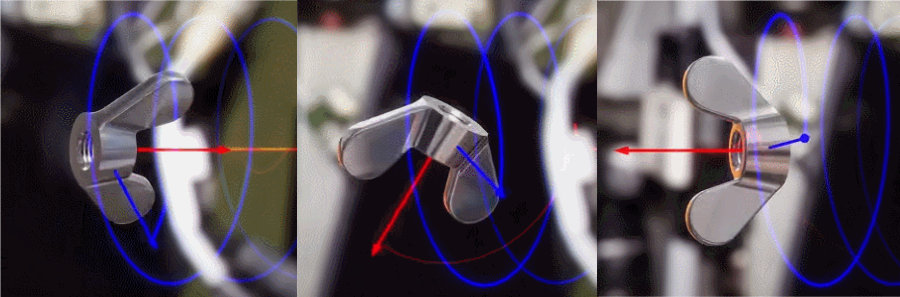
\includegraphics[width=0.9\textwidth]{dzhani.jpg}
\end{center}
   \caption{系绳效应的示意图 \cite{28}。}
\label{fig:10}
\end{figure*}

地球自转轴快速改变的原理在于旋转物体的物理学。经典的例子是由俄罗斯宇航员 Vladimir Dzhanibekov 发现的系绳效应 \cite{37},如图 \ref{fig:10} 所示。一个未能完美地围绕其三个主惯性轴之一旋转的物体将无法保持固定的自转轴。如果在离其第二主惯性轴不远的情况下旋转,它将经历看似突然的旋转变化。虽然这并不是我们认为地球快速翻转时发生的确切情况,但重点是在没有外部力的情况下,只有旋转物理学可以解释地球自转轴的快速变化。

准确地说,地球几乎可以肯定不会经历简单和一致的系绳效应。如果是这种情况,我们将能够检测到地球自转轴随时间的逐渐变化。相反,我们认为地球经历了周期性突发性体质结构变化,导致了其“外部旋转” (地壳/地幔)和“内部旋转体” (地核)的解耦。在没有外部输入的情况下,角动量守恒定律表明地球不能突然改变自转轴,因此外部和内部旋转体的解耦是唯一能导致突然翻转的少数因素之一,除非地球受到外部冲击。

地球内部破坏的具体过程被认为是地球核心铁结构的状态变化(图\ref{fig:11})。内核由六方密堆积铁 (Fe) 组成 \cite{141}。当这种 hcp-Fe 被转化为液态金属状态时,它释放出动能,并被诱导进入外核。该相变减少了核心的磁导率,削弱了地磁场,并释放热量,形成了地幔中的 LLVP(大型低速剪切区域)结构(图\ref{fig:12})\cite{38},通过深海加热地球表面。最近几个世纪中,这两种趋势已被很好地记录,并将在本文后面进行讨论。

\begin{figure}[t]
\begin{center}
   \includegraphics[width=1\linewidth]{llvp.jpg}
\end{center}
   \caption{南非下方 LLVP 的详细视觉 \cite{28}。}
\label{fig:12}
\label{fig:onecol}
\end{figure}

\begin{figure*}[t]
\begin{center}
\includegraphics[width=1\textwidth]{layers.jpg}
\end{center}
   \caption{导致 ECDO 翻转的地球内部过程的描述 \cite{129}。}
\label{fig:11}
\end{figure*}

\begin{figure*}[b]
\begin{center}
\includegraphics[width=0.9\textwidth]{saa.jpg}
\end{center}
   \caption{从 1590 年到 2025 年的地磁场削弱的描述。使用 gufm1 和 IGRF-14 模型计算 \cite{125,126}。}
\label{fig:14}
\end{figure*}

地球内部同样的过程,相反地被认为也驱动了地球翻转后不久恢复到当前旋转状态。

\section{即将到来的地球翻转的证据}

有充分理由相信我们正处在另一次地球翻转的边缘。数千年来没有发生大灾变,这大约是根据历史记载和数据这些事件似乎发生的频率。支持即将翻转的最有力的数据来自最近的地磁数据,表明地球的地磁场大约在两千年来一直在削弱。这种削弱正在加速并在过去几十年中达到了惊人的速度。

图\ref{fig:14}展示了1590年和2025年的地球地磁场 \cite{125,126}。如图所示,场强大幅减弱。

地磁场减弱的另一个指标是地磁北极的位置(图\ref{fig:13})。长期以来,地磁北极一直位于加拿大北极。然而,在过去的几个世纪中,它一直在缓慢游移,并在几十年前显著加速。它现在正以每年55公里的速度快速向俄罗斯移动 \cite{124}。

\begin{figure}[t]
\begin{center}
   \includegraphics[width=1\linewidth]{npw.jpg}
\end{center}
   \caption{1590年至2025年地磁北极位置,每5年增量描述 \cite{142}。}
\label{fig:13}
\label{fig:onecol}
\end{figure}

\begin{figure}[t]
\begin{center}
   \includegraphics[width=1\linewidth]{ocean-highlight.jpg}
\end{center}
   \caption{1991年到2010年深(>2000米深度)海洋变暖率,红色圆圈标出 \cite{132}。}
\label{fig:15}
\label{fig:onecol}
\end{figure}

地球的磁场被认为由内部发电机产生 - 因其旋转在地球外核中运动的圆柱形岩浆流 \cite{123}。地磁场的减弱是地球内部深处扰动的症状。根据 ECDO 理论,这些扰动会排出热量,并最终导致地幔和核心的解耦,从而导致地球翻转 \cite{1}。

有大量数据证实地球内部存在放热过程。地球变暖体现在大陆和海洋表面温度的上升 \cite{127,128}、大气中CO2水平的上升与地球热羽流同步 \cite{129,130},以及全球海冰范围的减少 \cite{131}。数据表明,CO2水平和温度的上升不是“人为”气候变化的原因,而是放热核心的下游效应 \cite{129}。

最显著的是,深海(深度 $>$2000 米)变暖速率的研究表明,不仅深海在变暖,最强的变暖速率出现在深渊层(4000 - 6000 米)。这种深海变暖的中心在4000米以下 \cite{132,129},如果海洋是被大气从上方加热,这种情况就不可能发生。这些数据强烈支持近期气候和地磁变化是由地球内部深处的过程驱动的观点。图 \ref{fig:15} 描绘了1991到2010年全球深海变暖速率 \cite{132}。

\section{地球即将翻转的建模}

\begin{figure}[b]
\begin{center}
   \includegraphics[width=1\linewidth]{saa-crop.jpeg}
\end{center}
   \caption{基于南大西洋异常的一个临界点计算得出日期为2059年3月13日 \cite{125,126}。}
\label{fig:16}
\label{fig:onecol}
\end{figure}

预测地球下一次翻转的时间是一个复杂的任务。目前,我们对此的最佳模型在于地球的地磁场——南大西洋异常区(SAA)。此区域位于南大西洋,具有最弱的地磁场强度,定义为场强低于32000纳特的区域 \cite{135},这一数值在1590年是最弱的。南大西洋异常区的表面积从1590年占地球表面的1%增加到2025年的21% \cite{136}。

为了估算地球可能翻转的时间,我将SAA表面积数据拟合到一个描述复杂系统接近关键转换点的幂律临界点方程上,该转换点是系统经历剧烈和突然变化的时刻。我的计算得出一个预测的临界点日期为2059年3月13日(图 \ref{fig:16})。随着我们越来越接近该转换,这一预测将变得越来越准确 \cite{136}。

其他指标如旋转轴漂移、天气异常以及地震和火山数据也可以帮助我们更好地预测下一次地球翻转可能发生的时间。

\section{ECDO历史时间线}

尽管确定过去ECDO事件的确切时间线很困难,但似乎在全新世期间至少发生了2次ECDO事件。请注意希罗多德从埃及祭司那里得到的记述,\textit{"从第一任国王到这位赫淮斯托斯的祭司末代国王,已历经三百四十一世代的人... 在这个时间里,他们说太阳四次从它惯常的升起地点移动,到他现在升起的地方,他曾两次在那里有过他的升起,并从他现在升起的地方,曾有过他的两次落下"} \cite{32}。柏拉图生活在公元前五世纪 \cite{111},他提到在9000年前,一天一夜之间淹没了亚特兰蒂斯的洪水之后,\textit{"自此之后,已发生了许多次洪水,逃到山上的幸存者不识文字,多世代以来完全致力于获得生活手段"} \cite{112},这表明自约公元前9700年末次冰期年轻德里亚斯以来发生了不止两次翻转。本文和我的研究 \cite{2} 中所涵盖的实物证据提供了大量证明柏拉图的说法的证据。

候选ECDO翻转的最近日期是公元前2300年至1600年期间,许多灾难性洪水记载(鲧禹 \cite{113,114,115},奥吉格斯 \cite{116,117},秘鲁 \cite{118,119},出埃及记 \cite{120})、文明的毁灭和废弃(摩亨佐-达罗 \cite{121},米诺斯克里特\cite{100,101})和物理异常(博德事件 \cite{122},4.2千年事件 \cite{90})都被归于此期。没有充足的更近期的证据汇聚来表明发生了一场重大灾难性事件。

\section{结论}

NANOOK行动是冷战时期美国的一次侦察行动,旨在二战后绘制北极和北苏联海岸的地图 \cite{137}。在他们的调查中,他们发现磁极比以前的探险发现的位置要靠北125到200英里。因此,\textit{"在政府科学家中,出现了一个问题,即磁极和地理极重合时会发生什么。为了回答这个问题,在保罗·A·西普尔博士的项目控制下,兰德公司被委托进行实验室研究,使用由同心球体构成的地球模型进行研究——一个内球体代表电磁荷的地球熔融铁核,其轴定义了“磁”极;一个外球体代表地壳,围绕“地理”极轴旋转。通过反复实验确定,当“磁”极接近“地理”极时,“磁”极在某一点会加快汇聚速度,仿佛被向“地理”极的向心力吸引而跳跃重合;但极未重合,“磁”极会迅速绕“地理”极“翻转”,然后仿佛受到了离心力的作用,转向赤道,最终两个轴线约形成89度的偏离。在发生了极“翻转”后,这些轴线会逐渐开始在很长时间内重新汇聚"} \cite{138,139}。

随后,\textit{"在1948年初,怀特少校参加的五角大楼的一次科学会议上,科学家们讨论了是否应向公众警示即将发生的极翻转现象。没有科学家同意将信息从公众中隐瞒;但另一方面,他们也无法就如何公布信息达成一致。某些人认为,这一现象的知识本身可能会摧毁社会的道德纤维。他们的恐惧显然是没有根据的,因为在1950年代初,有关翻转现象的信息被发布在一篇报纸专栏和一篇杂志文章中,但令人惊讶的是,显然震惊的、狭隘的或难以置信的公众没有产生任何反应"} \cite{138,139}。

为什么我们没有关注这一点?有充分的理由相信地球过去曾翻转过。本文及其第二部分提供了来自许多领域的大量证据汇聚的总结,表明情况可能如此,例如世界范围内的洪水故事,覆盖大陆的盐和海洋化石,古老的地下庇护所,动物遗骸和灾难性地质景观。人类据说已经存在了数十万年,而现代历史却只有几千年的记载。是否可能每隔一段时间,地球翻转,大陆被清除,我们被迫回到起点——石器时代——将古代历史的记录减少到为数不多的灾难性故事?如果是这样,那么防止这种情况再次发生可能是人类最重要的任务之一。

最后,我将留下佳篇,选自柏拉图所著的《蒂迈欧篇》,讲述了雅典政治家梭伦与埃及祭司之间的对话 \cite{140}:\textit{“在某个场合,[梭伦] 想引导他们讨论古代历史,于是他试图讲述我们最古老的传说,关于据说是第一个人的福洛纽厄斯和尼俄柏的故事;然后他继续讲述洪水后的丢卡利翁和皮拉的传说,以及他们如何幸存下来,并叙述他们后代的世系;通过列出所涉及事件所占用的年份,他试图计算时间段。其间一位祭司,一个极其年迈的人,说道:“啊,梭伦,梭伦,你们希腊人永远都是孩子:并不存在年老的希腊人。” 听到这话,他问道,“你这话是什么意思?” 祭司回答道,“你们每个人的灵魂都是年轻的。因为在你们之中,没有一个信仰是古老的,不是源自旧的传统,也没有一门学科是久远的。这就是其中的原因:曾经,而且将来会有许多种毁灭人类的方法,其中最大的毁灭是由于火和水引起的,而较小的则通过数不尽的其他手段造成。其实在你们国家与我们的国家传说中都有这样的故事:从前的某个时候,赫利俄斯的儿子法厄同驾驭着他父亲的战车,由于他无法沿着其父亲所走的路线行进,烧尽了所有在地上的东西,而他自己则被雷电击毙——那个故事,如今看来,是一个传说的形式,但其真实性存在于天空中围绕地球旋转的天体发生变动,以及地球上事物因猛烈的火灾而被毁灭的事实,并且此种事态以长间隔出现。每到这种时候,住在山上和高而干燥的地方的人比接近河流或海洋的人遭受更多的毁灭;而在我们这里,尼罗河在其他时候是我们的救世主,在这些时刻也通过上涨高度拯救了我们避免这场灾难。而当相反,诸神用洪水净化地球时,所有在山里的牧人和羊倌得以幸存,但那些在你们国家城市里的则被洪水卷入大海;然而在我们国家,无论是在那时还是在其他任何时刻,水都不会从上而下侵袭我们的田地,相反,它都自然地从下涌出。因此,正是由于这些原因,这里所保留的被认为是最古老的;事实是,每一个地方,只要无过度的热或寒能够阻碍,总有人类存在,只是人数时多时少而已。如果有任何高尚或伟大或引人瞩目的事件发生,不论是在你们国家还是在我们国家,或是我们通过传闻而知晓的其他地方,所有这样的事件都从古时起被记录并保存在我们的庙宇中;而你们的人和其他人每次都是新装备的,拥有书写字母和所有文明国家所需要的艺术,然而在经过通常的几年间隔之后,如同瘟疫一般,来自天上的洪水再次袭来,留下的只有文盲与未开化者,所以你们如同往常般年轻,毫不知晓在这个国家或你们自己的国家曾发生过的一切。诚然,刚才你所讲述的世系,梭伦,关于你们国家的人民,几乎只是孩童的故事;首先,你只记得一次洪水,虽然以前发生过许多次;其次,你不了解在你们现在所居住的地方曾孕育出人类中最崇高和最完美的种族,而你自己和你们现有的整座城市都是从某些偶然遗留的小种子中繁衍而来的;但你没有注意到这一点,因为在许多代中倖存者死去而没有能力用文字表达自己。确实,梭伦,在最大规模的水灾之前,有一段时间,现在的雅典国家在战争中最勇敢,并且在所有其他方面也是无比优秀的。有记载称它拥有人间所知最辉煌的艺术作品和最崇高的政体”。}
这些祭司当然也告诉梭伦关于亚特兰蒂斯古代文明的事:\textit{“对于我们这里来说,坐落在我们所说的海口之内,显然是一个有着狭窄入口的避风港;而那边是一个真正的海洋,环绕它的陆地可以被最公正地称为整个意义上的大陆。现在在这亚特兰蒂斯岛上存在一个国王的联合体,拥有巨大的而又惊人的力量,统治着整个岛屿,以及许多其他岛屿和大陆的一部分;而且,在海峡这边的土地上,他们统治着从利比亚至埃及,以及从欧洲至提尔赫尼亚的地区。因此,这支部队集结在一起,曾试图通过一次突袭来奴役你们的国家、我们的国家以及海峡内的整个领土。然后,就是在那时,梭伦,你们国家的男儿在全世界面前展现出了非凡的勇气和力量。因为它以勇敢和所有的战争艺术卓然领先,并且部分担任希腊人的领袖,部分在被其他人抛弃时独自屹立,在面临最致命的危险后,挫败了入侵者并树立了纪念碑;因此,它解救了那些尚未被奴役的人,以及所有住在赫拉克勒斯疆域内的其他人,无私地给予了自由。但在此后的某个时期,发生了可怕的地震和洪水,在一个悲惨的日夜降临时,你们的所有战士都被大地吞噬,亚特兰蒂斯岛也同样被大海吞没,消失无踪”。}

\section{致谢}

感谢Ethical Skeptic,ECDO论文的原创作者,完成了他富有洞察力、开创性的论文并与世界分享。他的三部分论文\cite{1}仍然是外核-地幔解耦詹尼别科夫振荡(ECDO)理论的重要著作,其中包含了比我在此简短介绍的更多关于该主题的信息。

感谢Ankit,他处理了表1中的灾难编译数据。

当然,感谢我们所站在的巨人;正是他们所做的所有研究和调查使得这项工作成为可能,并努力为人类带来光明。

\clearpage
\twocolumn

\section{附加图片}

\begin{figure}[H]
\begin{center}
   \includegraphics[width=1\linewidth]{wave.jpg}
\end{center}
   \caption{近距离观察哈夫拉金字塔上的底切抛物线波侵蚀\cite{27}。}
\label{fig:19}
\label{fig:onecol}
\end{figure}

\begin{figure}[H]
\begin{center}
   \includegraphics[width=1\linewidth]{star-stone.jpg}
\end{center}
   \caption{在胡夫金字塔的一个通道中刻在石头上的星图\cite{28}。}
\label{fig:20}
\label{fig:onecol}
\end{figure}

\begin{figure*}[t]
\begin{center}
\includegraphics[width=1\textwidth]{deepsea.jpg}
\end{center}
   \caption{深海和深海底加热异常与正常大气海洋加热曲线的对比视觉效果。整体加热异常来自NOAA \cite{147},深海和深海底加热分布来自Desbruyeres研究\cite{132},数据处理和可视化由Ethical Skeptic完成\cite{129}。}
\label{fig:21}
\end{figure*}

\begin{figure*}[t]
\begin{center}
\includegraphics[width=1\textwidth]{sealevel.jpeg}
\end{center}
   \caption{海平面显示出75年间63个站点的方差增加了20\%,表明洋流速度增加。海平面方差的激增与海洋热脉冲同时发生,表明这些可能都是由地球深海以下的加热引起的\cite{2,129}。}
\label{fig:22}
\end{figure*}
\begin{figure*}[t]
\begin{center}
\includegraphics[width=1\textwidth]{co2.jpg}
\end{center}
   \caption{大气中的二氧化碳浓度在过去的45年中持续上升,可能是由于海洋温度的升高引起的。来源:NOAA \cite{148,129}。}
\label{fig:23}
\end{figure*}

\begin{figure*}[t]
\begin{center}
\includegraphics[width=1\textwidth]{ice.jpg}
\end{center}
   \caption{全球海冰范围在过去的45年中一直在缩小,这归因于地球变暖。来源:ADS \cite{149}。}
\label{fig:24}
\end{figure*}

\clearpage
\twocolumn

{\small
\bibliographystyle{ieee}
\bibliography{egbib}
}

\end{document}
